\documentclass{article}
\usepackage[T1]{fontenc}
\usepackage{lmodern}
\usepackage{graphicx}
\usepackage{amsmath,amssymb}
\usepackage[a4paper,margin=2cm]{geometry}
\usepackage[absolute,overlay]{textpos}
\setlength{\TPHorizModule}{1mm}
\setlength{\TPVertModule}{1mm}
\usepackage[indonesian]{babel}
\usepackage{hyperref}
\setlength{\emergencystretch}{2em}
% unit: Halaman 76

\begin{document}

% === Halaman 76 (llm) ===

3. Jika dua huruf tidak pada baris yang sama atau kolom yang sama, maka:\
\begin{itemize}
    \item huruf pertama diganti dengan huruf pada perpotongan baris huruf pertama dengan kolom huruf kedua.
    \item huruf kedua diganti dengan huruf pada titik sudut keempat dari persegi panjang yang dibentuk dari tiga huruf yang digunakan sampai sejauh ini.
\end{itemize}

\vspace{10mm}

\begin{center}
    Bigram: hz\\
    \vspace{5mm}
    Cipherteks: BW
\end{center}

% deskripsi: Tabel matriks huruf untuk metode enkripsi Playfair yang menunjukkan proses pencarian ciphertext untuk bigram 'hz', dengan panah merah yang menghubungkan huruf H, B, dan Z untuk membentuk persegi panjang.
% bbox normalisasi: [0.3570, 0.5600, 0.5670, 0.9050]
\begin{textblock*}{44.10mm}(74.97mm,166.32mm)
\noindent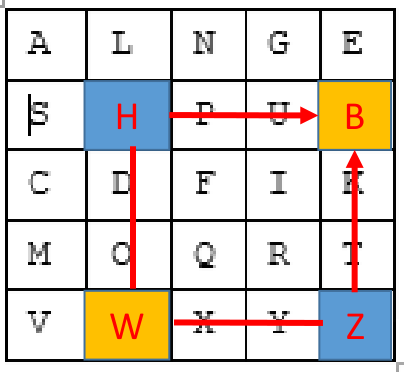
\includegraphics[width=44.10mm,height=102.46mm]{../../images/llm/page_076_img_01.png}%
\end{textblock*}

\end{document}
